\documentclass[12pt]{article}
\usepackage[utf8]{inputenc}
\usepackage[margin=1.0in]{geometry}

\title{GADMA user manual \\ \normalsize  Corresponding to version 1.0.0}
\author{Ekaterina Noskova}
\date{}

\usepackage{graphicx}
\usepackage{siunitx}
\usepackage{amsmath}
\usepackage{enumerate}
\usepackage{xspace}
\newcommand{\dadi}{$\partial$a$\partial$i\xspace}
\newcommand{\moments}{\textit{moments}\xspace}
\usepackage{hyperref}
\usepackage{listings}
\newcommand{\py}[1]{\lstinline[language=Python, showstringspaces=False]@#1@}
\usepackage{csquotes}
\lstset{
basicstyle=\ttfamily,
language=Bash,
showstringspaces=False,
%aboveskip=0pt,
captionpos=b,
%belowskip=0pt
}

\usepackage[title]{appendix}

\begin{document}

\maketitle
\tableofcontents
\clearpage


\section{Introduction}
Welcome to GADMA!\\

GADMA implements methods for automatic inferring the joint demographic history of multiple populations from genetic data.

GADMA is based on two open source packages: \dadi developed by Ryan Gutenkunst [\url{https://bitbucket.org/gutenkunstlab/dadi/}] and \moments developed by Simon Gravel [\url{https://bitbucket.org/simongravel/moments/}].

In contrast, GADMA is a command-line tool. It presents a series of launches of the genetic algorithm and infers demographic history from the Allele Frequency Spectrum of multiple populations (up to three).

\subsection{Getting help}
If you have any problems or questions, please don't hesitate to contact me by email:\\ \textbf{ekaterina.e.noskova@gmail.com}. I will be glad to answer your questions. 

\section{Parameter file}

A parameter file is a simple text file (created in a text editor, such as Notepad), which contains a list of parameters and variables with their assigned values. Create a parameter file that reflect your particular parameters. Hereinafter, as an example, the name of your parameter file will be defined as \py{param_file}.

\section{Hands on}

\paragraph{Test case}\mbox{}\\
GADMA has a test case for a simple demographic model for one population: just a constant size of $10000$ individuals in population. To run a test case:

\begin{lstlisting}
$ gadma --test
\end{lstlisting}

\paragraph{Example 2}\mbox{}\\
Suppose we have SNP data for two populations. Data is in \dadi's SNP file format in the \py{snp_data.txt}. Suppose we want to get all output in some \py{gadma_output} directory:


\begin{lstlisting}
$ gadma -i snp_data.txt -o gadma_output
\end{lstlisting}


\paragraph{Example 3}\mbox{}\\
We didn't specify AFS size or labels for populations, they are taken automatically from the input file. We can see a parameter file of our run in the \py{gadma_output/param_file}. 
\begin{lstlisting}
# gadma_output/param_file
...
Population labels : pop_name_1, pop_name_2
Projections: 18, 20
...
\end{lstlisting}
But we know that spectrum should be $20 \times 20$! To specify size of AFS we need to create a parameter file and set \py{Projections}:

\begin{lstlisting}
# param_file
Projections : 20,20
\end{lstlisting}

Order of populations can be changed as:
\begin{lstlisting}
# param_file
Projections : 20,20
Population labels : pop_name_2, pop_name_1
\end{lstlisting}

If we want to rename populations, we should change names on \py{snp_data.txt} file.

Now assume we want to get the simplest demographic model as fast as we can. We will tell GADMA that we need no other dynamics of population sizes except sudden (constant) population size change and that we want to use \moments library.

\begin{lstlisting}
# param_file
Projections : 20,20
Population labels : pop_name_2, pop_name_1
Only sudden : True
Use moments or dadi : moments
\end{lstlisting}

To run GADMA we need to specify \py{-p/--params} command-line option in cmd:
\begin{lstlisting}
$ gadma -i snp_data.txt -o gadma_output -p params_file
\end{lstlisting}

\paragraph{Example 4}\mbox{}\\
Consider some AFS file \py{fs_data.fs}. There is a spectrum for three populations: YRI, CEU, CHB. However axes are mixed up: CHB, YRI, CEU. To run GADMA we should order them from most ancient to most recent:
\begin{lstlisting}
# param_file
Population labels : YRI, CEU, CHB
\end{lstlisting}

We want to allow exponential growth (it is the default behaviour) and have some extra changes in size of the ancient population. To do so we should specify \py{Initial structure}. It is list of three numbers: first --- number of time intervals before first split (we want here 2); second --- number of time periods between first and second split events (at least 1); third --- number of time periods after second split.

\begin{lstlisting}
# param_file
Population labels : YRI, CEU, CHB
Initial structure : 2,1,1
\end{lstlisting}

Also we can put information about input file and output directory to our parameter file:
\begin{lstlisting}
# param_file
Input file : fs_data.fs
Output directory : gadma_output
Population labels : YRI, CEU, CHB
Initial structure : 2,1,1
\end{lstlisting}

Now we can run GADMA in the following way:
\begin{lstlisting}
$ gadma -p params
\end{lstlisting}

\paragraph{Example 5}\mbox{}\\
We have our GADMA launch interrupted for some reasons. We want to resume it:
\begin{lstlisting}
$ gadma --resume gadma_output
\end{lstlisting}
where \py{gadma_output} is output directory of previous run. We can find resumed run in \py{gadma_output_resumed}

\paragraph{Example 6}\mbox{}\\
Our launch was finished, we used \dadi with a default grid size which GADMA determines automatically if it is not specified by user. We found out that it would be better to find some models using greater number of grid points in \dadi scheme, but we want to take final models from previous run:

\begin{lstlisting}
# param_file
Pts : 40, 50, 60 #Greater value of grid size than it was
\end{lstlisting}

And run GADMA:
\begin{lstlisting}
$ gadma --resume gadma_output --only_models -p params 
\end{lstlisting}

\py{--only_models} tell GADMA to take from \py{gadma_output} final models only. \\

There is another way to do the same:
\begin{lstlisting}
# param_file
Resume from : gadma_output
Only models : True
Pts : 40, 50, 60 #Greater value of grid size than it was
\end{lstlisting}

And run GADMA in the following way:
\begin{lstlisting}
$ gadma -p params
\end{lstlisting}

\paragraph{Example 7}\mbox{}\\
We can add a custom model using a parameter \py{Custom filename} in the parameter file:

\begin{lstlisting}
# param_file
Custom filename : YRI_CEU_demographic_model.py
\end{lstlisting}

Our custom file need to contain a function with a fixed name \py{model_func} (see Appendix A). For example:

\begin{lstlisting}
# YRI_CEU_demographic_model.py
def model_func((nu1F, nu2B, nu2F, m, Tp, T), (n1,n2), pts)
    xx = yy = dadi.Numerics.default_grid(pts)

    phi = dadi.PhiManip.phi_1D(xx)
    phi = dadi.Integration.one_pop(phi, xx, Tp, nu=nu1F)

    phi = dadi.PhiManip.phi_1D_to_2D(xx, phi)
    nu2_func = lambda t: nu2B*(nu2F/nu2B)**(t/T)
    phi = dadi.Integration.two_pops(phi, xx, T, nu1=nu1F, 
                                    nu2=nu2_func, m12=m, m21=m)

    sfs = dadi.Spectrum.from_phi(phi, (n1,n2), (xx,yy))
    return sfs
\end{lstlisting}

In addition, we can easily specify values for lower and upper bounds through a parameter file. Let's set lower and upper bounds for the model we defined above:

\begin{lstlisting}
# param_file
Lower bounds : 1e-2, 1e-2, 1e-2, 0, 0, 0
Upper bounds : 100, 100, 100, 10, 3, 3
\end{lstlisting}

\paragraph{Example 8}\mbox{}\\
Also, we can get the values of lower/upper bounds, both, or none of them in the parameter file automatically. For this, each identifier in the parameter file must be declared through a parameter \py{Parameter identifiers}. Below is an identifier list:

\begin{lstlisting}
# param_file
#   An identifier list:
#   T - time
#   N - size of population
#   m - migration
#   s - split event, proportion in which population size
#   is divided to form two new populations.
\end{lstlisting}

For example, we set a lower bound for the model we defined above (see Example 7) and we want to get an upper bound automatically.

\begin{lstlisting}
# param_file
Lower bound : 1e-2, 1e-2, 1e-2, 0, 0, 0
Upper bound : None

Parameter identifiers : n, n, n, m, t, t
\end{lstlisting}

\paragraph{Example YRI, CEU}\mbox{}\\
GADMA has an example of the parameter file \py{example_params} that is presented \hyperref[sec:example-params]{at the end of the manual}. To run GADMA with this parameters one should just run from the GADMA's home directory:
\begin{lstlisting}
$ gadma -p example_params
\end{lstlisting}


\section{Input data}

GADMA supports several types of input data, which are familiar to anyone who has used \dadi or \moments in the past:
\begin{itemize}
    \item Frequency spectrum file format (.fs or .sfs),
    \item SNP data format (.txt).
\end{itemize}
Input file can be specified to GADMA in two ways:

\begin{enumerate}
    \item Through command-line option \py{-i/--input}:
\begin{lstlisting}[language=bash]
  $ gadma -i fs_file.fs -o out_dir
\end{lstlisting}
  or
\begin{lstlisting}
  $ gadma --input snp_file.txt -o out_dir
\end{lstlisting}
    \item Use a parameter \py{Input file} in the parameter file:
    
  \begin{lstlisting}
  # param_file
    
  # Input file path
  Input file : fs_file.fs 
  ...
  \end{lstlisting}
\end{enumerate}    
Extra information about input AFS can also be put in the parameter file. For example, AFS can be projected to a smaller size with \py{Projections} option, populations can be named or their order can be changed with \py{Population labels} option. If parameter file does not contain some options, they are automatically pulled out from the input file.
    
\begin{lstlisting}
# param_file
    
# Input file path
Input file : fs_file.fs
    
# (New) size of the AFS
Projections : 20,20
    
# Labels of populations
Population labels : CEU, YRI
...
\end{lstlisting}
GADMA can be launched with a parameter file in the following way:
\begin{lstlisting}
$ gadma -p params_file -o out_dir
\end{lstlisting}



\subsection{VCF data format}
To convert a VCF (.vcf) file into a SFS (.sfs) file use \url{https://github.com/isaacovercast/easySFS}.

\subsection{Frequency spectrum file format}

Each file begins with any number of comment lines beginning with \py{\#}.
The first non-comment line contains $P$ integers giving the dimensions of the FS array, where $P$ is the number of populations represented.
For a FS representing data from 4x4x2 samples, this would be \py{5 5 3}.
(Each dimension is one larger than the number of samples, because the number of observations can range, for example, from 0 to 4 if there are 4 samples, for a total of 5 possibilities.)
On the same line, the string \py{folded} or \py{unfolded} denoting whether or not the stored FS is folded.

The actual data is stored in a single line listing all the FS elements separated by spaces, in the order fs[0,0,0] fs[0,0,1] fs[0,0,2]\dots fs[0,1,0] fs[0,1,1]\dots.
This is followed by a single line giving the elements of the mask in the same order as the data, with \py{1} indicating masked and \py{0} indicating unmasked.

\subsection{SNP data format}

\begin{lstlisting}[caption={Example of SNP file format}, label={lst:SNP_data}]
Human Chimp Allele1 YRI  CEU  Allele2 YRI CEU Gene  Position
ACG   ATG   C       29   24   T       1   0   abcb1 289
CCT   CCT   C       29   23   G       3   2   abcb1 345
\end{lstlisting}

The data file begins with any number of comment lines that being with \py{#}.
The first parsed line is a column header line.
Whitespace is used to separate entries within the table, so no spaces are allowed within any entry.
Individual rows make be commented out using \py{#}.

The first column contains the in-group reference sequence at that SNP, including the flanking bases.
If the flanking bases are unknown, they can be denoted by \py{-}.
The header label is arbitrary.

The second column contains the aligned outgroup reference sequence at that SNP, including the flanking bases.
Unknown entries can be denoted by \py{-}.
The header label is arbitrary.

The third column gives the first segregating allele.
The column header must be exactly \py{Allele1}.

Then follows an arbitrary number of columns, one for each population, each giving the number of times Allele1 was observed in that population.
The header for each column should be the population identifier.

The next column gives the second segregating allele.
The column header must be exactly \py{Allele2}.

Then follows one column for each population, each giving the number of times Allele2 was observed in that population.
The header for each column should be the population identifier, and the columns should be in the same order as for the Allele1 entries.

Then follows an arbitrary number of columns which will be concatenated with \py{_} to assign a label for each SNP.

The \py{Allele1} and \py{Allele2} headers must be exactly those values because the number of columns between those two is used to infer the number of populations in the file.

~\
\subsection{Unlinked SNP's}

By default, SNP's that were used to build AFS are considered to be linked. In this case it is possible to compare demographic models with different number of parameters by Composite Likelihood Akaike Information Criterion ($CLAIC$). This procedure can be necessary as a model with a large number of parameters will be better able to find parameter values corresponding to the observed data than a model with a smaller number of parameters, but at the same time it will correspond less to reality, for example, due to data errors. It is called overfitting and we do not want it to happen.

Actually, $CLAIC$ is modification of usual Akaike Information Criterion ($AIC$), but $AIC$ can be used only for AFS built from unlinked SNP's. The smaller the $AIC$ or $CLAIC$ score is, the better the model fits the observed data.

It is possible to inform GADMA about linkage of SNP's and unlock the usage of $AIC$ insted of $CLAIC$:

\begin{lstlisting}
# param_file

# Inform if SNP's are not linked
Linked SNP's : False
...
\end{lstlisting}

~\
\section{Specifying a scheme}

GADMA uses either \dadi or \moments to simulate expected AFS from the demographic model. \dadi is used by default. To use \dadi it is recommended to check the value of the \py{Pts} option in the \py{params_file}. \py{Pts} is sequence of three numbers, each of which is equal to the number of points in grid size. The greater the numbers are, the more accurate \dadi numerical solution of partial differential equation is. However, finding such a solution take more time. By default, GADMA takes \py{Pts : n, n + 10, n + 20}, where \py{n} — is the largest sample size among populations of interest. 

\moments library does not need \py{Pts} to be specified. To change \dadi to \moments scheme, specify option in the parameters file:

\begin{lstlisting}
# param file
...
Use moments or dadi : moments
...
\end{lstlisting}

\section{Specifying a model}

\subsection{Dynamics of population size change}
\begin{figure}[hb!]
  \centering
  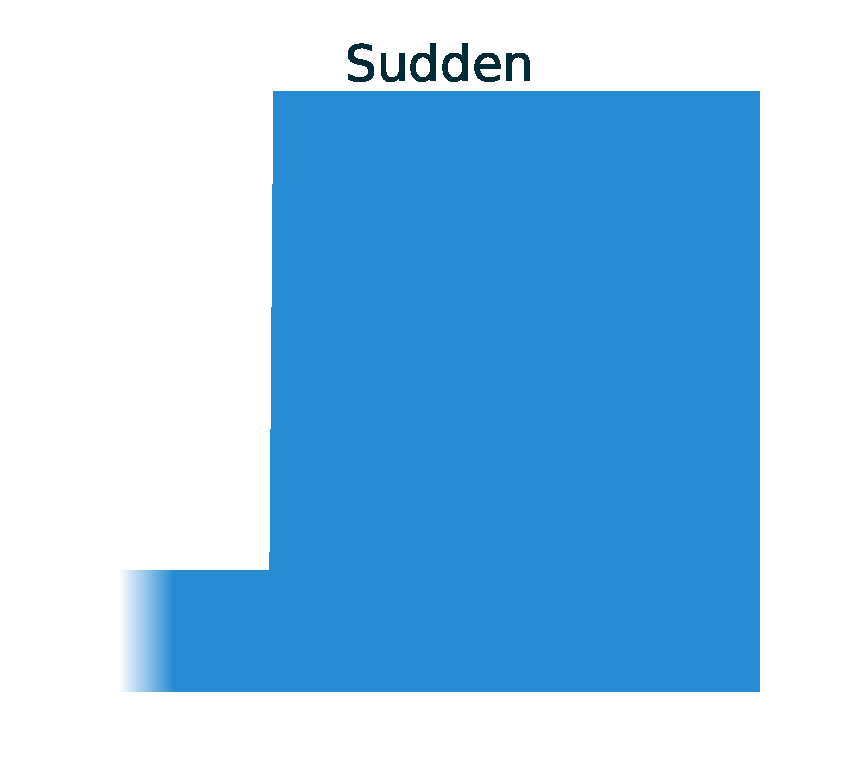
\includegraphics[width=0.25\linewidth] {sudden.eps}
  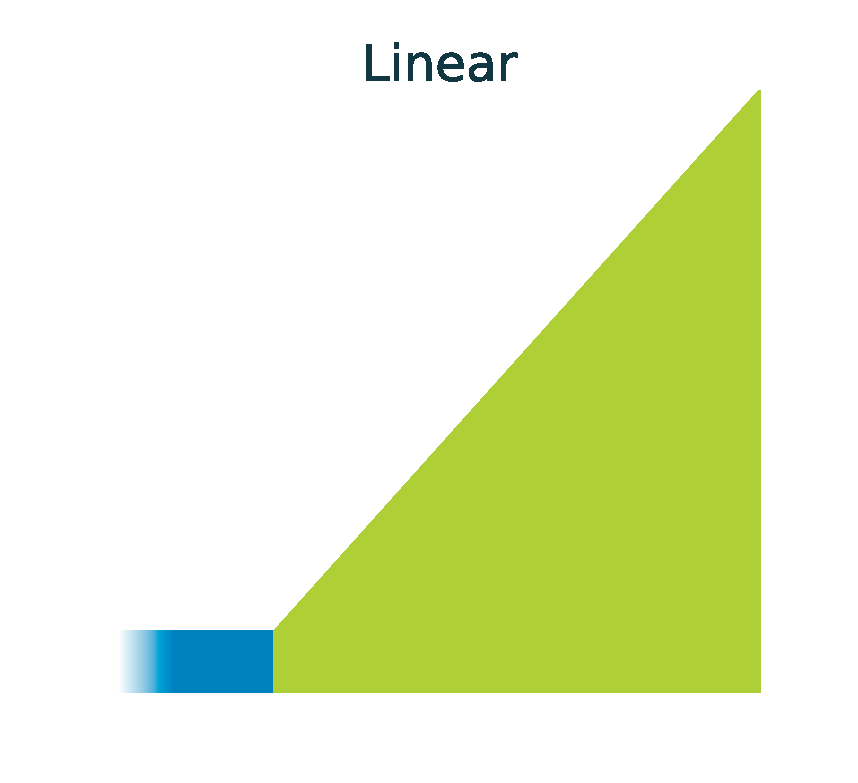
\includegraphics[width=0.25\linewidth] {linear.eps}
  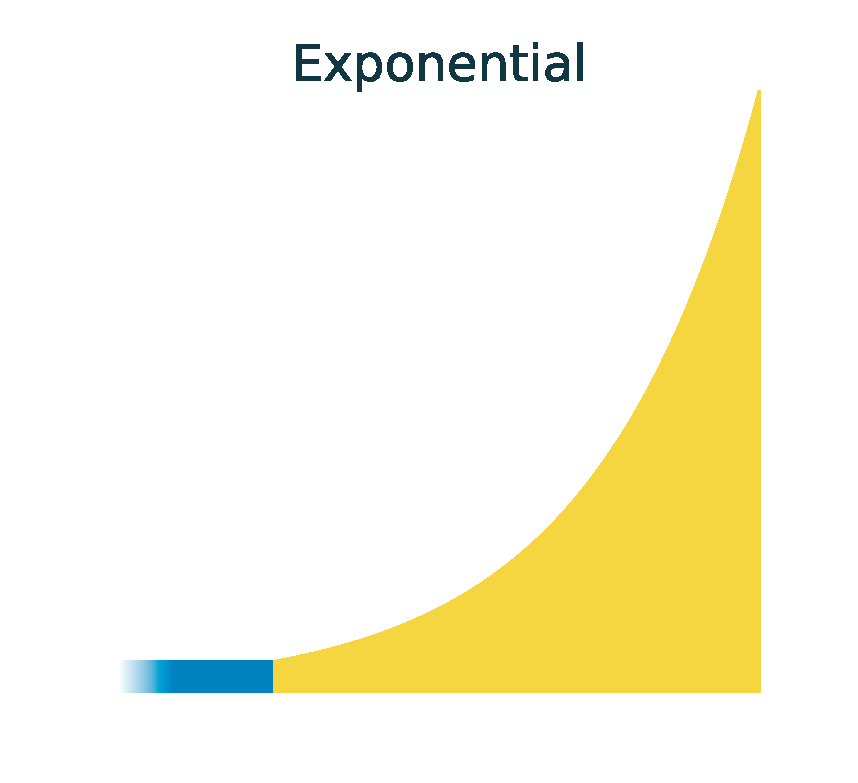
\includegraphics[width=0.25\linewidth] {exponential.eps}
  \caption{Three main demographic dynamics of population size change.}
  \label{fig:laws_of_size_change}
\end{figure}
In GADMA the size of population can be changed due to one of three dynamics: sudden change, linear change and exponential change of the effective population size (Figure~\ref{fig:laws_of_size_change}). 

In order to infer a demographic model with sudden changes of populations sizes only, option \py{Only sudden} in the parameters file should be set to \py{True}:

\begin{lstlisting}
# param_file
...
Only sudden : True
...
\end{lstlisting}
By default, this option is set to \py{False} and dynamics are found like other parameters of the demographic model.

\subsection{Specifying the structure of the model}

GADMA infers a demographic model from an AFS with nothing required from the user, except simple information, that determines how much the detailed model is required --- \textbf{the structure of the model}.

Assume a division of one population into two new subpopulations and a fixed temporal order of the populations: from the most anciently to the most recently formed population. 

We can divide time of our model into split events and time intervals, during which a certain dynamics of change of effective size is maintained for each population and migration rates are constant. The number of split events is one less than the number of populations under consideration. Now we can define the concept of the structure of the demographic model:

\textbf{Structure of the demographic model is}:
\begin{itemize}
    \item the number of time intervals in case of one population;
    \item the number of time intervals as those that occur before and after a single split, in the case of  two populations;
    \item the number of time intervals prior to the first split, those between the first and second split, and the ones after the second split, in the case of three populations.
\end{itemize} 

\begin{figure}[b!]
  \centering
  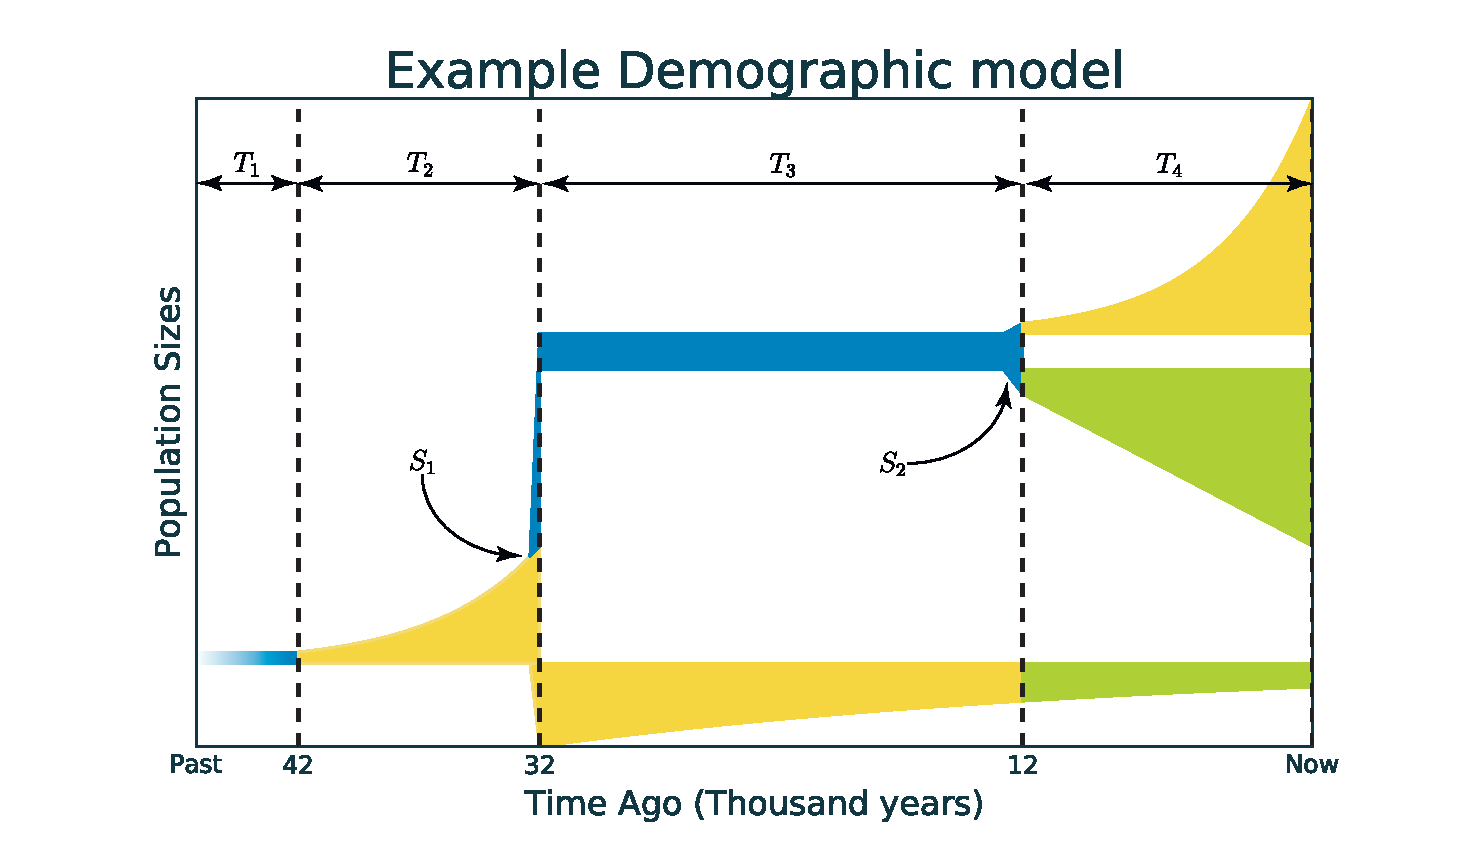
\includegraphics[width=0.7\linewidth]{dem_model_col.eps}
  \caption{Example of representation of demographic model. Time is on the axis of abscissa and population size is on the axis of ordinates. The structure of that model is (2,1,1). The colours reflect different demographic dynamics.}
  \label{fig:exaple_of_model_plot}
\end{figure}

For example, we can divide into time of the model on the Figure~\ref{fig:exaple_of_model_plot} to four time intervals: $T_1$, $T_2$, $T_3$ and $T_4$, and two populations' splits: $S_1$ and $S_2$. The structure of this model is $2,1,1$, because two intervals ($T_1$ as $T_2$) before first split $S_1$, one interval ($T_3$) between first and second splits and one interval ($T_4$) after second split $S_2$.

\subsubsection{Initial structure}
To specify the structure of the inferred model one should set \py{Initial structure} in the parameter file:

\begin{lstlisting}
    # param_file
    ...
    Initial structure : 2
    ...
\end{lstlisting}
or
\begin{lstlisting}
    # param_file
    ...
    Initial structure : 2,1
    ...
\end{lstlisting}
or
\begin{lstlisting}
    # param_file
    ...
    Initial structure : 2,1,1
    ...
\end{lstlisting}
By default the simplest structure is used (1 or 1,1 or 1,1,1).

\subsubsection{Final structure}
It is also possible to start with a simpler structure in order to get to a more complex one. To do so one should specify option \py{Final structure} in the parameter file. For example:

\begin{lstlisting}
# param_file
Input file : some_2d_fs.fs
    
Initial structure : 1,1
Final   structure : 2,1
...
\end{lstlisting}
Within this parameter file GADMA will find parameters for demographic model with 1,1 structure, then increase structure  2,1 and find parameters for the model with this structure. Parameters identify within a more simple structure (in this case it is 1,1) are used further to define the parameters of a more complex structure (2,1).

\textbf{Note:} Structure increases random, so if one specifies initial structure to 1,1 and final to 2,2, it is not guaranteed to final optimal parameters for demographic models with structures between 1,1 and 2,2, i.e. intermediate state can be either 1,2 or 2,1.

\textbf{Recommendation:} Use scheme with a more complex structure, as it produce more stable solutions.

\textbf{Recommendation:} Choose recommended values for model's structure. Final structure should differ by one element from initial structure, for example, 1,1 and 2,1; 1,2,1 and  2,2,1.


\subsection{Specifying a model in details}
\label{sec:spec-model-in-det}

It is also possible to use Genetic algorithm from GADMA to a proposed model that is defined as Python function using \dadi or \moments. It is the way that \dadi and \moments work with demographic models inference. To understand how to specify a model like that one can read manuals to the packages. 

For example, consider simple bottleneck model for one population: at time \py{TF + TB} in the past, an equilibrium population goes through a bottleneck of depth \py{nuB}, recovering to relative size \py{nuF}:

\begin{lstlisting}
def bottleneck(params, ns, pts):
    nuB, nuF, TB, TF = params
    xx = dadi.Numerics.default_grid(pts)
    
    phi = dadi.PhiManip.phi_1D(xx)
    phi = dadi.Integration.one_pop(phi, xx, TB, nuB) 
    phi = Integration.one_pop(phi, xx, TF, nuF)
    
    fs = dadi.Spectrum.from_phi(phi, ns, (xx,)) 
    return fs
\end{lstlisting}

To run optimization from GADMA one needs to run optimization function just like in \dadi and \moments:

\begin{lstlisting}
# Import GADMA's optimization function:
import gadma

# Specify input data and its parameters:
data = dadi.Spectrum.from_file("fs_filename.fs")
ns = data.sample_sizes # size of AFS
pts = [40,50,60] # grid size for dadi

# Wrap our bottleneck function:
func_ex = dadi.Numerics.make_extrap_log_func(bottleneck)

# Specify upper and lower bounds for parameters:
upper_bound = [100, 100, 3, 3]
lower_bound = [1e-2, 1e-2, 0, 0]

# Run optimizations:
 run the optimization 
# Beginning GADMA optimization
popt = gadma.Inference.optimize_ga(4, data, func_ex, pts_l,
                                   p_ids = ['n', 'n', 't', 't'],
                                   lower_bound=lower_bound,
                                   upper_bound=upper_bound)
# Beginning local optimization from dadi
popt = dadi.Inference.optimize_log(popt, data, func_ex, pts_l,
                                   lower_bound=lower_bound,
                                   upper_bound=upper_bound,
                                   verbose=len(p0), maxiter=3)

print('Found parameters: {0}'.format(popt))
\end{lstlisting}

\textbf{Note:} As GADMA optimization is a global search algorithm, no initial parameters \py{p0} are set in \py{gadma.Inference.optimize_ga} function. However, it is possible to specify \py{p0}:
\begin{lstlisting}
# Initial parameters can be set too:
p0 = [0.01, 1.5, 0.2, 0.2]

# Beginning GADMA optimization
popt = gadma.Inference.optimize_ga(4, data, func_ex, pts_l, p0=p0, 
                                   p_ids = ['n', 'n', 't', 't'],
                                   lower_bound=lower_bound,
                                   upper_bound=upper_bound)
\end{lstlisting}
If one wants to find other parameters for \py{gadma.Inference.optimize_ga} function:

\begin{lstlisting}
>>> import gadma
>>> help(gadma.Inference.optimize_ga)
\end{lstlisting}

\section{Several repeats and parallel computing}

By default, GADMA runs optimization that uses Genetic algorithm once. However, it is recommended to run optimization several times and choose the best model among the resieved ones. Option \py{Number of repeats} in the parameter file tells GADMA how many times an optimization should be executed. Moreover, there is another option \py{Number of processes} that allows GADMA to run all the processes in parallel. 

\textbf{Note:} GADMA parallelize exactly several runs, not every of them. So if one asks to repeat optimization twice and parallelize in more than 2 processes, only two processes will be used eventually. 

\textbf{Recommendation:} \py{Number of processes} should be less than \py{Number of repeats} and it will be better if it is aliquot to the \py{Number of repeats}.

\textbf{Note:} \py{Number of processes} shouldn't be greater than the number of kernels on one's computer. Otherwise there will be no sense in parallelization.

\begin{lstlisting}
# param_file
...
Number of repeats : 6
Number of processes : 2 # or 3 or 6
...
\end{lstlisting}

\section{Output}
GADMA puts all files to the directory that user set through \py{-o/--output} command-line option:
    \begin{lstlisting}
    $ gadma -o output_dir -i input_fs.fs
    \end{lstlisting}
or through \py{Output directory} option in the parameter file:
    \begin{lstlisting}
    # param_file
    ...
    Output directory : output_dir
    ...
    \end{lstlisting}

\subsection{Stdout and log file}
GADMA prints its progress about every minute in stdout and in \py{output_dir/GADMA.log} file:

\begin{lstlisting}
[hhh:mm:ss]
All best logLL models:
GA number       logLL            AIC             Model

All best AIC models:
GA number       logLL            AIC             Model

--Best model by log likelihood--
Log likelihood:       	Best logLL
with AIC score:         AIC_score
Model: 	representation of best logLL model

--Best model by AIC score--
Log likelihood:       	logLL
with AIC score:         Best AIC score
Model:  representation of best AIC model 
\end{lstlisting}
 
\textbf{Note:} One can set \py{Silence} option in the parameter file to \py{True} to disable output in stdout, file \py{output_dir/GADMA.log} will still have it.

\subsection{Model representation}
Every model is printed as a line of parameters. All model parameters, except mutation rates, have precision equaled to 2.

Consider designations:
\begin{itemize}
    \item \py{T} --- time,
    \item \py{P} --- percent of split,
    \item \py{Ni} --- size of population number \py{i},
    \item \py{di} --- dynamic of changing of the size of population number \py{i},
    \item \py{mij} --- mutation rate from population \py{i} to population \py{j}.
\end{itemize}

Dynamic of population size change has numerical values: 
\begin{itemize}
    \item \py{di = 0} --- sudden change of size for population number \py{i};
    \item \py{di = 1} --- linear change of size for population number \py{i};
    \item \py{di = 2} --- exponential change of size for population number \py{i}.
\end{itemize}

Model is printed as sequence of time intervals and splits that are represented in the following way:

\begin{itemize}
    \item First period (\py{NA} --- size of ancestry population):

\py{[ NA ]}

    \item Split:
    \begin{itemize}
        \item If there are one population before split event, so there will be two populations after it:

\py{[ P\%, [N1, N2] ]}
        
    \item If there are two population before split event, so last formed population is divided and there will be three populations after it:

\py{[ P\%, [N1, N2, N3] ]}

    \end{itemize}
    \item Usual time period:
    \begin{itemize}
        \item If there is one population:

\py{[ T, [N1], [d1] ]}

        \item If there are two populations:

\py{[ T, [N1, N2], [d1, d2], [[None, m12], [m21, None]] ]}

        \item If there are three populations:

\py{[ T, [N1, N2, N3], [d1, d2, d3],}

\hspace{2cm} \py{[[None, m12, m13], 
[m21, None, m23], [m31, m32, None]] ]}

    \end{itemize}

\end{itemize}

At the end of the string, that corresponds to the model, there is an information about model's ancestry in the genetic algorithm: 
\begin{itemize}
    \item \py{c} --- for model, that is child of crossover,
    \item \py{r} --- if it was formed random way,
    \item \py{m} --- if it was mutated,
    \item \py{f} --- final model of genetic algorithm.
\end{itemize}

\textbf{Note:} \py{m} is added as many times as model is mutated.\\

\textbf{Example of the demographic model for two populations}:

\py{[ [144.38] ][ 16.00\%, [23.10, 121.28] ][ 375.77, [143.31, 30.07],}

\hspace{6cm} \py{ [2, 2], [[None, 3.33e-03][7.53e-04, None]] ]}


\subsection{Output directory content}

For every repeat of Genetic algorithm GADMA creates a new folder in output directory with corresponding number.

In every folder there is \py{GADMA_GA.log}, where every iteration of algorithm is saved, folders \py{pictures} and \py{python_code}.

When genetic algorithm finishes GADMA saves picture and python code of received model in the corresponding folder.

When all GA's are executed, the codes are saved in the root directory.
\begin{lstlisting}
- <output_dir>
	- 1
		GADMA_GA.log
		- pictures
		- python_code
			- dadi
			- moments
		result_model.png
		result_model_code.py
	- 2
		GADMA_GA.log
		- pictures
		- python_code
			- dadi
			- moments
		result_model.png
		result_model_code.py
	params
	extra_params
	GADMA.log
	best_logLL_model.png
	best_logLL_model_dadi_code.py
	best_logLL_model_moments_code.py
	best_aic_model.png
	best_aic_model_dadi_code.py
	best_aic_model_moments_code.py
\end{lstlisting}

\subsection{Generated code of models}


By default, GADMA generates python code only for final models both for \dadi and \moments. However, it can do it every $N$ iteration of genetic algorithm. In this case option \py{} should be set in the parameter file. GADMA saves files with code to the \py{output_dir/<GA_number>/python_code} directory. Both \dadi and \moments code are generated and saved in different folders there. 

Each code contains function of the model, which takes values of the parameters as input, and strings that load observed AFS, simulates expected AFS from the model's function and calculates log likelihood between two AFS'. The result log likelihood is printed to stdout. For the \moments code picture is also drawn.

All codes can be run in the following way:
\begin{lstlisting}
$ python file_with_code.py
\end{lstlisting}

Example of generated code one can find at the end of this manual in \hyperref[sec:ex-gen-code]{the corresponding section}.

\section{Plotting model}

\begin{figure}[h]
    \centering
    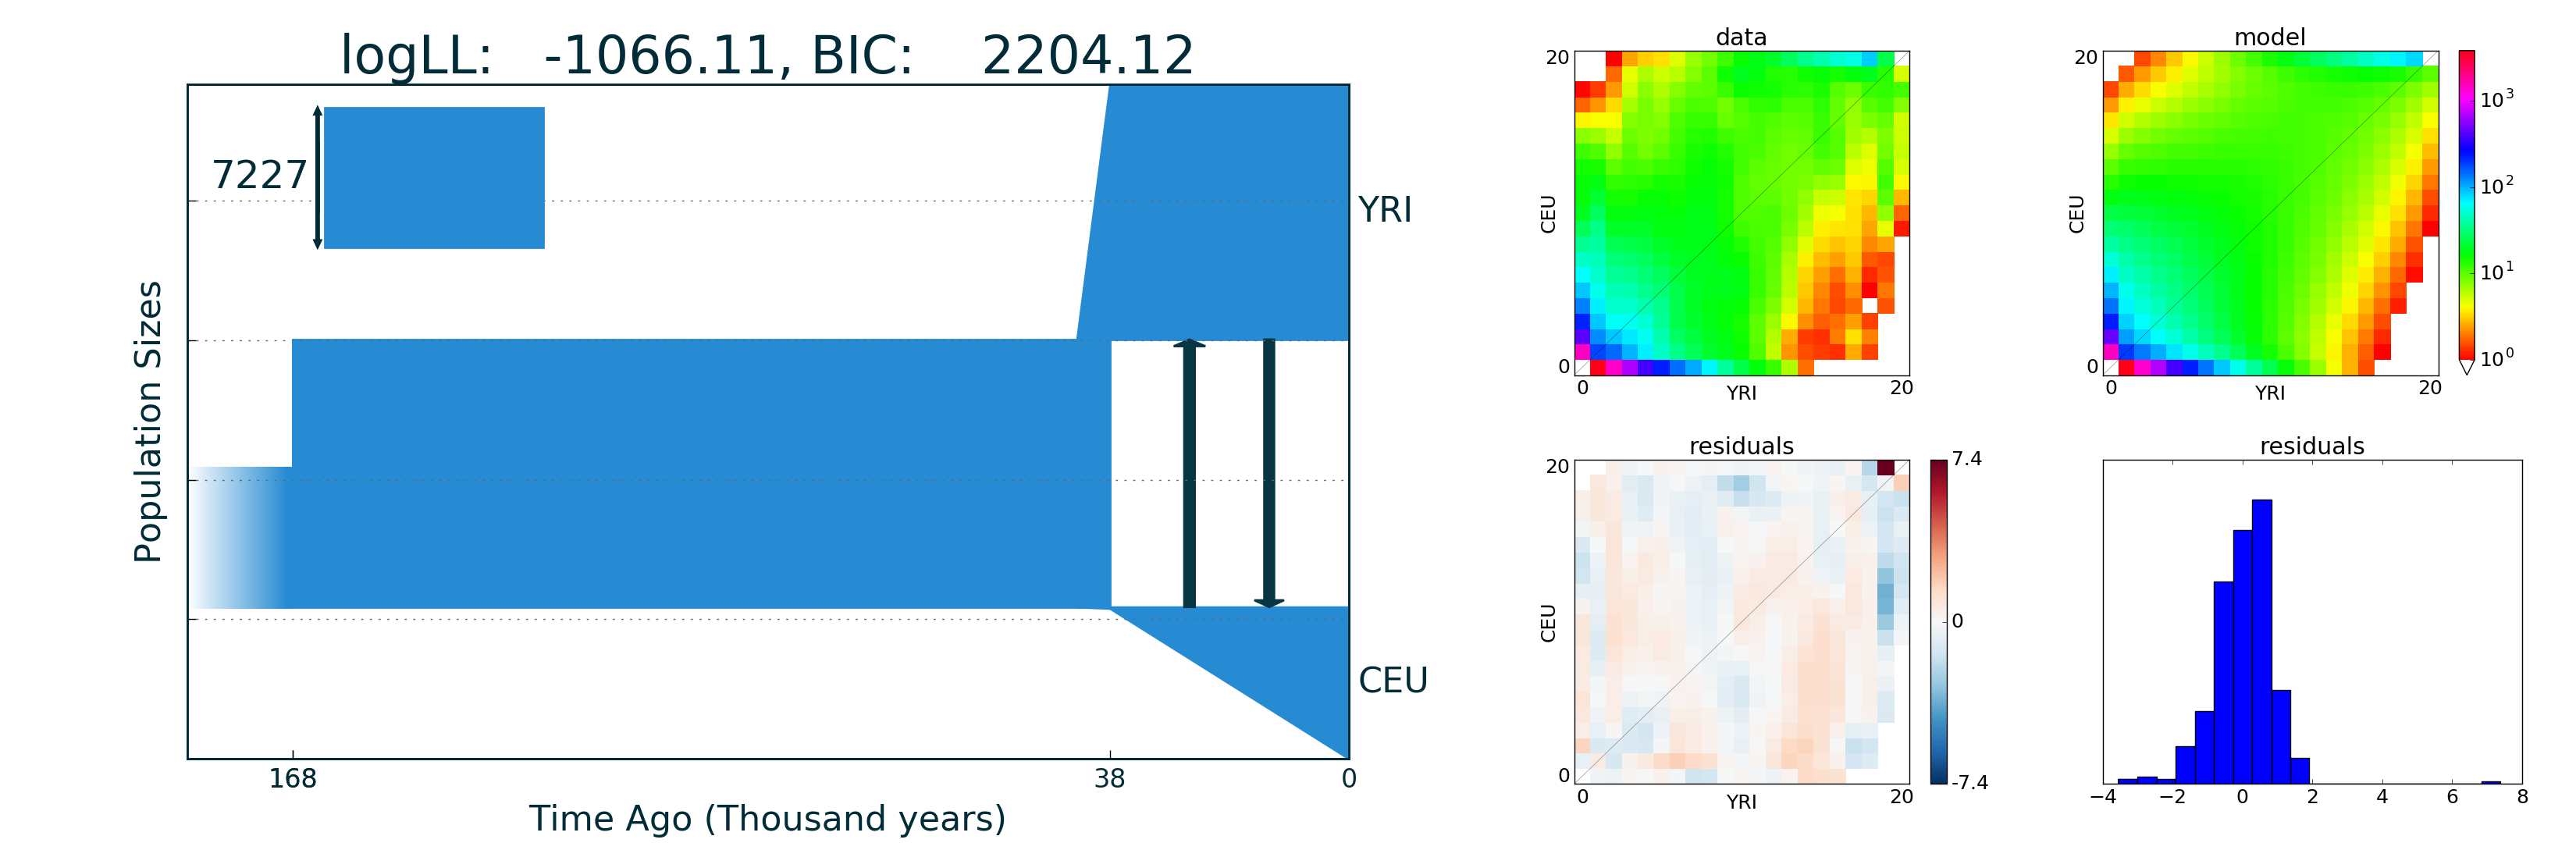
\includegraphics[width=\linewidth]{example_model_plot.png}
    \caption{Example of demographic model plot that GADMA draws during run.}
    \label{fig:my_label}
\end{figure}

GADMA always draws final best models during genetic algorithms search for best solutions.

However, models can be drawn during the pipeline every $N$'s iteration of each genetic algorithm. $N$ is equal to the value of \py{Draw models every N iteration } option in the parameter file. So to enable drawing one should set this option in file.

\textbf{Recommendation:} Don't draw models very often, because changes are usually not very significant and drawing takes some time, so optimization will be slower.

\textbf{Note:} One can disable drawing by setting \py{Draw models every N iteration : 0 } in the parameter file. This is also default behaviour.

Models are drawn with \moments library, so it should be installed if one wants to have pictures. In the top left corner there is a size of ancestry population. Other parameters one can find in string representation of the model in the log files.

\subsection{Time units on model's plot}
Time on the demographic model's plot can be drawn in units of years,  thousand years or in genetic units. By default choice depends on the \py{Time for generation} option in the parameter file: if it is set to some value (in years) then time will be shown in years, otherwise it will be in genetic units.

But, of course, it is possible to tell GADMA which units are preferable. For example, if one wants time to be in thousands of years on the pictures, as it is a big value in years:

\begin{lstlisting}
# param_file
...
Units of time in drawing : thousand years
...
\end{lstlisting}

\subsection{Plotting after GADMA finished}

\begin{figure}[h]
    \centering
    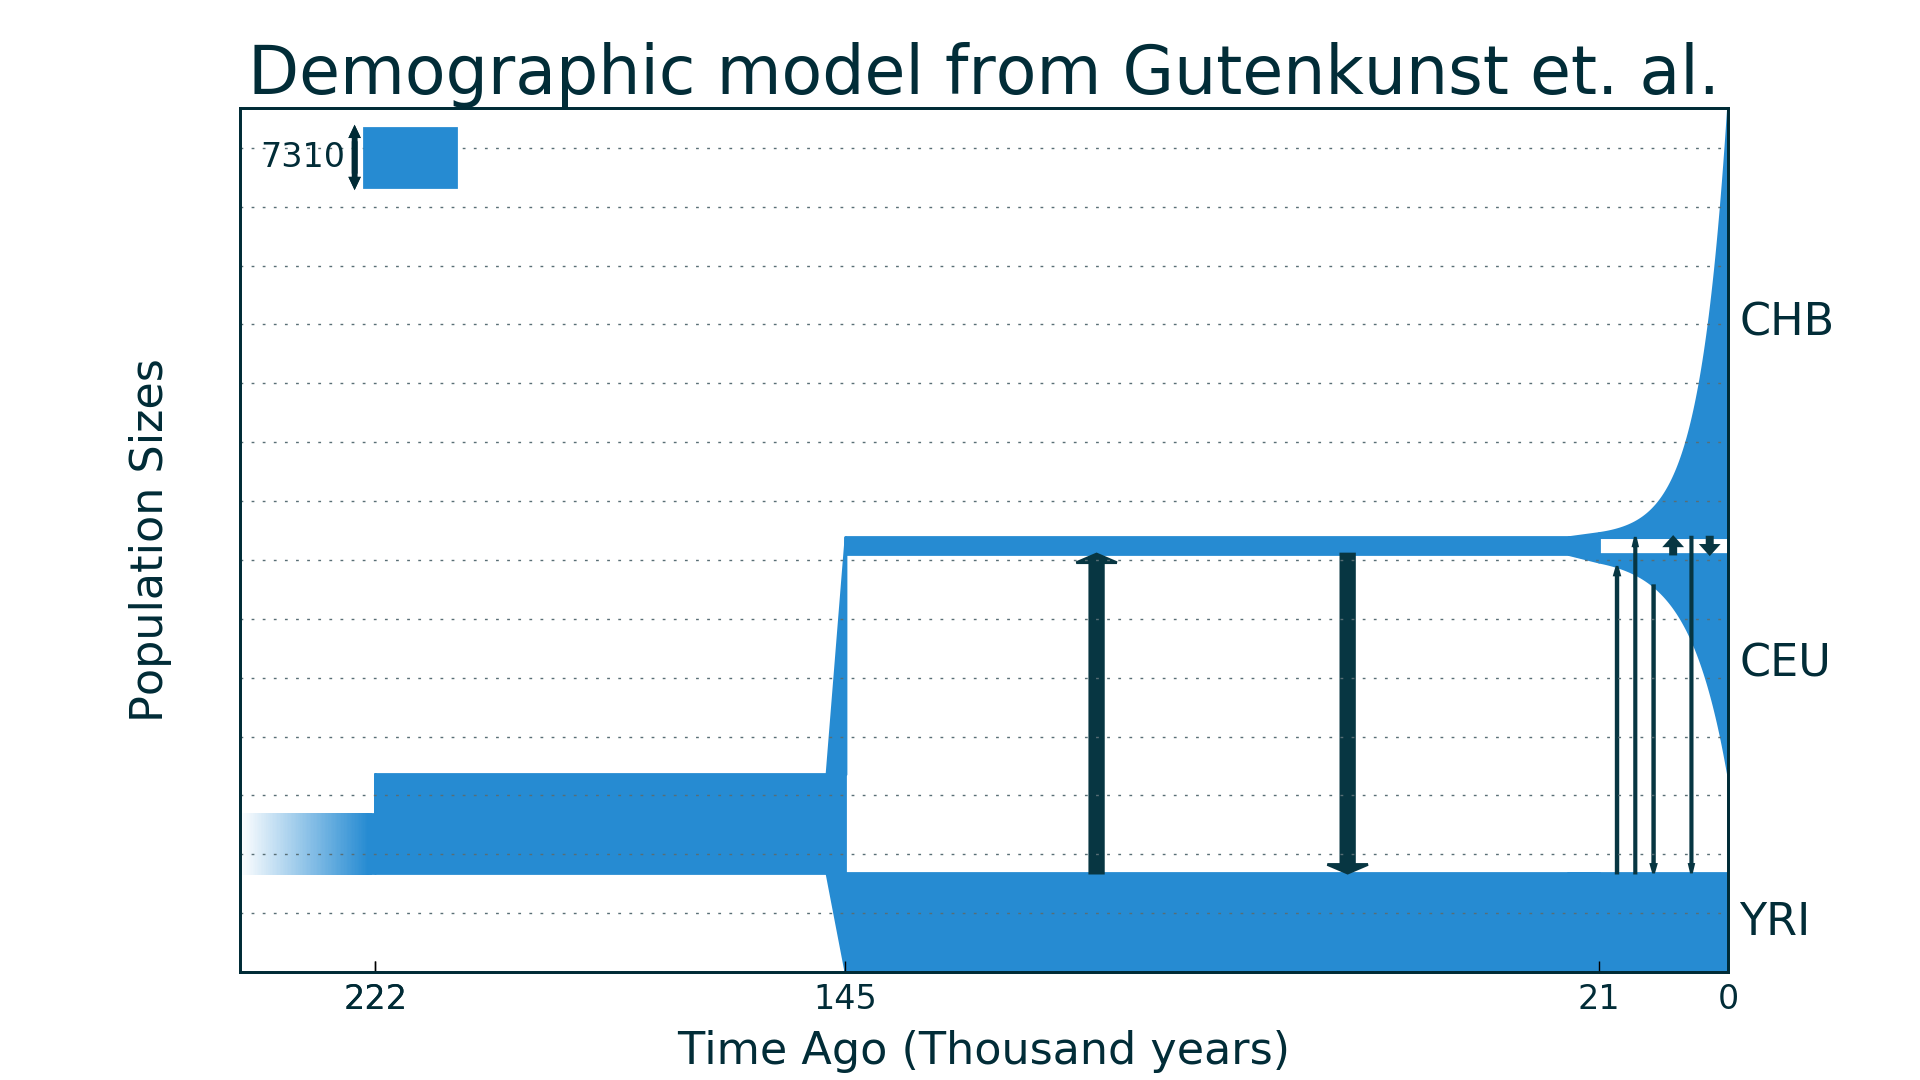
\includegraphics[width=0.6\linewidth]{3d_lim_model_dadi.png}
    \caption{Example of model's plot that was drawn with generated python script.}
    \label{fig:my_label}
\end{figure}

Sometimes final pictures aren't satisfying or one didn't draw for some reasons (didn't want to install \moments, wanted fast launch) it is possible to plot demographic model (and only it) again.

To do it one should run corresponding generated python script for the model. For example, final model can be drawn again in the following way:
\begin{lstlisting}
$ python best_logll_model_moments_code.py
\end{lstlisting}

\textbf{Note:} Again it's possible only if one has \moments installed.

\textbf{Note:} One can change code inside the file and drawn again if picture isn't satisfying.

\section{Usefull options}
\subsection{Time for generation}
Option \py{Time for generation} in the parameter file is corresponding to the time per one generation in Wright-Fisher model. It is responsible basically for one thing: time on the model's plots. If it is specified, then time on the pictures will be converted from genetic units by scaling with this value. Otherwise, if it is not set, time will be shown in genetic units. 

\textbf{Note:} If \py{Time for generation} is specified, it should be consistent with another option: \py{Theta0}, which is described in \hyperref[sec:est-theta]{the corresponding section}.

\subsection{\py{Theta0}}
\py{Theta0} is equal to the expected number of mutations that occur in one chromosome in one generation in the infinite-sited model. GADMA can scale all values of demographic model parameters due to known value of \py{Theta0}. However, it is not always possible to find it. There is a way to solve this problem: one can set \py{Theta0} to \py{None} or just not specify it at all, so GADMA will take it as $1.0$ and after launch one can scale result values due to found \py{Theta0} (how to do it is described in the \hyperref[sec:change-theta]{corresponding section}). 

\subsubsection{Estimating \py{Theta0}}
\label{sec:est-theta}
If $\mu$ --- is the neutral mutation rate per site per generation and $L$ --- is the length of the sequence, then:

$$\theta_0 = 4 \cdot \mu \cdot L$$

\textbf{Note:} $L$ is the effective sequence length, which accounts for losses in alignment and missed calls.

\textbf{Note:} $\mu$ should be estimated based on generation time. One can leave \py{Time per generation} option in the parameter file unspecified (then time on the model's plots will be in the genetic units), but one should recalculate $\mu$! \\

\textbf{For example (Gutenkunst et al, 2009 \cite{gutenkunst2009})}:

\begin{displayquote}
We estimate the neutral mutation rate $\mu$ using the divergence between human and chimp. Comparing aligned sequences in our data, we estimate the divergence to be 1.13\%. Assuming a divergence time of 6 million years and a mean generation time for human and chimp over this interval of 25 years, we have

$$\mu = 0.0113 \cdot 25 / (2 \cdot 6 \cdot 10^6) = 2.35 \times 10^{-8}\text{ per generation}.$$
\end{displayquote}

\subsubsection{Changing \py{Theta0}}
\label{sec:change-theta}
If GADMA was launched with one \py{Theta0} and now one wants to use another or if it was launched with default \py{Theta0} $ = 1.0$ and now one has estimated its real value, model's parameters can be simply scaled:\\

Let  $a = \frac{\displaystyle \theta_0^{NEW}}{\displaystyle \theta_0^{OLD}},$
\begin{itemize}
    \item Size of population $/ a$,
    \item Time $/ a$,
    \item Migration rates $\cdot a$,
    \item Split percent stay the same.
\end{itemize}

\subsection{Examples of \py{Theta0} and time for generation}
The following tables produce different possible values for the demographic model inference for three populations of modern people: YRI, CEU, CHB.
\begin{table}[h]
    \centering
    \begin{tabular}{|l|c|c|c|c|l|}
        \hline
        FS filename	        & Gen. time  &	$\mu$	   &      $L$	   & \py{Theta0} \\
                            & (years)   & (per site per gen.)  & (base pair) & (per chr. per gen.)\\
        \hline
        YRI\_CEU\_CHB.fs	& 25 \cite{gutenkunst2009}   & $2.35 \cdot 10^{-8}$ \cite{gutenkunst2009} & $4.04 \cdot 10^6$ \cite{gutenkunst2009} & $0.37976$ \\
        YRI\_CEU\_CHB.fs	& 24 \cite{lapierre2017accuracy} & $2.26 \cdot 10^{-8}$ \cite{gutenkunst2009} & $4.04 \cdot 10^6$ \cite{gutenkunst2009} & $0.36521$ \\
        YRI\_CEU\_CHB.fs	& 29 \cite{Jouganous1549}	& $1.44 \cdot 10^{-8}$ \cite{Jouganous1549} & $4.04 \cdot 10^6$ \cite{gutenkunst2009} & $0.23270$ \\
        YRI\_CEU\_CHB.fs	& 24 \cite{lapierre2017accuracy} & $1.2 \cdot 10^{-8}$ \cite{Jouganous1549}  & $4.04 \cdot 10^6$ \cite{gutenkunst2009} & $0.19392$  \\
        \hline
    \end{tabular}
    \caption{Examples of different values of generation time and its influence on $\mu$ and \py{Theta0}}
    \label{tab:my_label}
\end{table}

In Gutenkunst et al. \cite{gutenkunst2009} generation time for human populations was equal to $25$ years and mutation rate $\mu$ was estimated as $2.35 \cdot 10^{-8}$. If one wants to change time for one generation to $24$ years, one needs to scale $\mu$: $\mu / 25 \cdot 24 = 2.26 \cdot 10^{-8}$.

In Jouganous et al. \cite{Jouganous1549} generation time was grater --- $29$ years and mutation rate was equal to $1.44 \cdot 10^{-8}$. To change generation time to $24$, one needs to change value of the mutation rate: $\mu_{NEW} = \mu / 29 \cdot 24 = 1.2 \cdot 10^{-8}$. \py{Theta0} is calculated then by the formula above.

\textbf{Note:} One can find FS files in \py{fs\_examples} directory.

\subsection{Relative to $N_A$ parameters}
Sometimes it is more important to see parameters scaled to $N_{ref} = N_A$. To tell GADMA shows models with scaled parameters, option \py{Relative parameters} should be set to \py{True}. By default, it is \py{False}. It is conveniently when \py{Theta0} is unknown.

\subsection{Disable migrations}
GADMA can to exclude migrations rates from optimization and consider them be equal to zero. In that case all migrations are disabled. One should set option \py{No migrations} to \py{True} in the parameter file.

\subsection{Upper bound for time split}
To limit time of some split one should specify option in the parameter file. Splits are numerated from the most ancient. So split 1 is split that occurred with ancient population and split 2 is next division of second population (exist only for three populations). There are two appropriate options: \py{Upper bound of first split} and \py{Upper bound of second split}.

One should translate time from years into genetic units, therefore divide it by $2 \cdot T_g$, where $T_g$ is time (in years) for one generation. For example, one wants to limit last split with 2000 years. Time for one generation is estimated as 24 years, then one should specify in the parameter file:
\begin{lstlisting}
# param_file
...
Upper bound of second split : 83.333
...
\end{lstlisting}

\subsection{Resume launch}
To resume interrupted launch one can use \py{--resume} command-line option or set \py{Resume from} in the parameter file. One needs to set output directory of previous run.

If neither \py{Output directory} or \py{-o/--output} is not specified, GADMA will continue evaluation in the directory: \py{<previous_output_dir>_resumed}.

\subsubsection{Only models}
GADMA can resume launch taking final models only from previous run. This means, that it is not resumption, but run from some initial values. It is useful, for example, when one has to run GADMA with some small grid size for dadi and then wants to restart it with greater number of grid points. To do so, one should set command-line option \py{--only_models} with \py{--resume} or specify \py{Only models} option in the parameter file to \py{True}.

\section{Extra parameter file}
GADMA take an extra parameter file as input. \textbf{However one probably do not need them}. Nevertheless, if one is interested, \py{extra_params_template} with all options and their descriptions can be found in \py{gadma} folder.

\section{Units}
GADMA shows model parameters in genetic units. To scale them from one should multiply migration rates by 2 only. Other units are as usual. In case when option \py{Relative parameters} is set to \py{True} one should first rescale from units of $N_{ref}$: sizes of populations and time --- multiply by \py{NA}, migration rates --- divide by \py{NA}.

\section{Decreasing the number of model's parameters}
There are several ways to decrease the number of demographic model's parameters in GADMA. The first way as it was discussed above, is to consider only sudden dynamics of population size changes (\py{Only sudden : True}). The second way to decrease the number of parameters is so-called multinom scheme: when at every step $N_A$ is chosen to fit the observed data best. This scheme leads to faster work of GADMA, however it is more possible to get stuck in local optima. To use it one should set option \py{Multinom} to \py{True} in the parameter file. The third way is to disable migration by setting \py{No migrations} to \py{True} in the parameter file.

The last and more reliable way to decrease the of model's parameters is to use GADMA optimization on the custom model written with \dadi or \moments (section \hyperref[sec:spec-model-in-det]{Specifying model in details}). However, it requires some extra work for user.

\newpage
\section{Installation}

One can try to install GADMA and all its possible dependencies via shell script from GADMA home directory the following way:
\begin{lstlisting}
$ ./install
\end{lstlisting}

If some problems occur please try to install GADMA by steps that are described below.

\subsection{Dependencies}
GADMA requires the following dependencies:
\begin{itemize}
    \item Python (2.5, 2.6, 2.7)
    \item NumPy ($\geq 1.2.0$)
    \item Scipy ($\geq 0.6.0$)
    \item \dadi ($\geq 1.7.0$) or \moments ($\geq 1.0.0$)
\end{itemize}
To draw demographic models install the following:
\begin{itemize}
    \item matplotlib ($\geq 0.98.1$)
    \item Pillow ($\geq 4.2.1$)
    \item \moments ($\geq 1.0.0$)
\end{itemize}

NumPy and SciPy can be installed via \py{pip}:
\begin{lstlisting}
$ python -m pip install numpy
$ python -m pip install scipy
\end{lstlisting}

\subsection{\dadi}
To install \dadi, run the following command in the work directory:

\begin{lstlisting}
$ git clone https://bitbucket.org/gutenkunstlab/dadi/
\end{lstlisting}

Then go to the \py{dadi} directory and install package:

\begin{lstlisting}
$ cd dadi
$ python setup.py install
\end{lstlisting}

To check \dadi's installation, use the command:

\begin{lstlisting}
$ python
>>> import dadi
\end{lstlisting}

\subsection{\moments}

To install \moments, go to the work directory and run:

\begin{lstlisting}
$ git clone https://bitbucket.org/simongravel/moments/
\end{lstlisting}

Cython can be installed using \py{pip}:
\begin{lstlisting}
$ python -m pip install --upgrade Cython
\end{lstlisting}

Also \moments requires \py{mpmath}, which can be installed via \py{pip}:
\begin{lstlisting}
$ python -m pip install mpmath
\end{lstlisting}

Then go to the \py{moments} directory and install package:

\begin{lstlisting}
$ cd moments
$ python setup.py install
\end{lstlisting}

To check \moments's installation, use the command:

\begin{lstlisting}
$ python
>>> import moments
\end{lstlisting}

\subsection{Pillow}

Install Pillow with \py{pip}:

\begin{lstlisting}
$ python -m pip install Pillow
\end{lstlisting}

To check Pillow's installation, use the command:

\begin{lstlisting}
$ python
>>> import PIL
\end{lstlisting}

\subsection{GADMA}
To download GADMA, go to the work directory and run:

\begin{lstlisting}
$ git clone https://github.com/ctlab/GADMA
\end{lstlisting}

Then go to the \py{GADMA} directory and install GADMA:
\begin{lstlisting}
$ cd GADMA
$ python setup.py install
\end{lstlisting}

Now one can run it like this:
\begin{lstlisting}
$ gadma --help
\end{lstlisting}

\subsubsection{Verifying installation}
To verify the installation, run a test:

\begin{lstlisting}
$ gadma --test
\end{lstlisting}

If the installation was successful, one will find the following information at the end:
\begin{lstlisting}
--Finish pipeline--

--Test passed correctly--
Thank you for using GADMA!
\end{lstlisting}

\newpage
\begin{appendices}
\section{Example of the parameter file}
\label{sec:example-params}
\begin{lstlisting}
#   It is a parameter file for GADMA software.

#   Lines started from # are ignored.
#   Also comments at the end of a line are ignored too.
#   Every line contains: Identifier of parameter : value.
#   If one wants to change some default parameters, one needs to
#   remove # at the beginning of a line and change corresponding
#   parameter.


#   Output directory to write all GADMA out.
#   One needs to set it to not existing or empty directory.
#   If it is resumed from other directory and output directory 
#   isn't set, GADMA will add '_resumed' for previous output 
#   directory.
Output directory : my_example_run


#   One can resume from some other launch of GADMA by setting
#   output directory of it to 'Resume from' parameter.
#   You can set again new parameters of resumed launch.
#Resume from : another_output_dir


#   If one wants to take only models from previous run set this 
#   flag. Then iterations of GA will start from 0 and values of
#   mutation rate and strength will be initial.
#   Default : None
Only models : None


#   Input file can be sfs file (should end with .fs) or 
#   file of SNP's in dadi format (should end with .txt).
Input file : fs_examples/YRI_CEU.fs


#   'Population labels' is sequence of population names (the same
#   names as in input file)
#   If .fs file is in old format then it would rename population 
#   labels that are absent.
#   It is necessary to put them in order from most ancient to less. 
#   (In case of more than two populations)
#   It is important, because the last of formed populations take
#   part in next split.
#   For example, if we have YRI - African population,
#   CEU - European population and CHB - Chinese population,
#   then we can write YRI, CEU, CHB or YRI, CHB, CEU 
#   (YRI must be at the first place)
#   Default: from input file
Population labels : CEU, YRI # we change populations order 
                             # (in input file YRI is first)


#   Also one can project your spectrum to less size.
#   For example, we have 80 individuals in each of three 
#   populations, then spectrum will be 81x81x81 and one can 
#   project it to 21x21x21 by set 'Projections' parameter 
#   to 20, 20, 20.
#   Default: from input file
Projections : None # will be 20, 20


#	Are SNP's linked or unlinked?
#	If they are linked, then Composite Likelihood Akaike
#	Information Criterion (CLAIC) will be used to compare models.
#	If they are unlinked, then usual Akaike Information Criterion 
#	(AIC) will be used.
#	Default: True
Linked SNP's : True




#   Now all main parameters:
#
#   Total mutation flux - theta.
#   It is equal to:
#   theta = 4 * mu * L
#   where mu - mutation rate per site per generation and 
#   L - effective sequenced length, which accounts for losses 
#   in alignment and missed calls.
#   Note: one should estimate mu based on generation time.
#   Default: 1.0
Theta0 : 0.37976 # the same as in Gutenkunst et al 2009


#   Time (years) for one generation. Can be float. 
#   It is important for drawing models. If one doesn't want to draw, 
#   one can pass it.
#   Default: 1.0
Time for generation : 25 # the same as in Gutenkunst et al 2009


#   Parameters for demographic models:
#
#   Use moments or dadi
#   Default: dadi
Use moments or dadi : moments


#   Use multinom scheme: N_A is not parameter for search, 
#   it is calculated through optimal_sfs_scaling.
#   Multinom scheme decrease number of parameter by one and 
#   is usually faster, however non multinom scheme usually 
#   finds better solutions.
#   Default: False
Multinom : False


#   If you choose to use dadi, please set pts parameter - number
#   of points in grid
#   Default: Let n = max number of individuals in one population, 
#   then pts = n, n+10, n+20
#Pts : 20, 30, 40


#   Using a custom demographic model.
#   Please, specify file with function named 'model_func' in it. 
#   So file should contain:
#   def model_func(params, ns, pts) in case of dadi
#   or
#   def model_func(params, ns) in case of moments
#   Default: None
Custom filename : None

#   Now one should specify either bounds or identifications 
#   of custom model's parameters. All values are in Nref units.
#   Lower and upper bounds - lists of numbers.
#   List of usual bounds:
#   N: 1e-2 - 100
#   T: 0 - 5
#   m: 0 - 10
#   s: 0 - 1
#   This bounds will be taken automatically if identifications are set.
#   Default: None
Lower bounds : None
Upper bounds : None
#   An identifier list:
#   T - time
#   N - size of population
#   m - migration
#   s - split event,  proportion in which population size
#    is divided to form two new populations.
#   Default: None
Parameter identifiers : None


#   Structure of model for one population - number of time periods 
#   (e.g. 5).
#   Structure of model for two populations - number of time periods
#   before split of ancestral population and after it (e.g. 2,2).
#   Structure of model for three populations - number of time periods
#   before first split, between first and second splits and after 
#   second split (e.g. 2,1,2).
#
#   Structure of initial model:
#   Default: all is ones - 1 or 1,1 or 1,1,1
Initial structure : 2,1


#   Structure of final model:
#   Default: equals to initial structure
#Final structure : 2,2


#   It is possible to limit time of splits.
#   Split 1 is the most ancient split.
#   !Note that time is in genetic units (2 * time for 1 generation):
#   e.g. we want to limit by 150 kya, time for one generation is 
#   25 years, then bound will be 150000 / (2*25) = 3000.
#
#   Upper bound for split 1 (in case of 2 or 3 populations).
#   Default: None
#Upper bound of first split : None


#   Upper bound for split 2 (in case of 3 populations).
#   Default: None
#Upper bound of second split : None


#	Print parameters of model in units of N_ref = N_A.
#   N_A will be placed in brackets at the end of string.
#   Default: False
Relative parameters : False


#   Disable migrations in demographic models.
#   Default: False
No migrations : false




#   Parameters for Genetic Algorithm.
#
#   Size of population of demographic models in GA:
#   Default: 10
Size of population in GA : 10


#   Fractions of current models, mutated models and crossed models 
#   to be taken to new population.
#   Sum of fractions should be <= 1, the remaining fraction is 
#   fraction of random models.
#   Default: 0.2,0.3,0.3
#Fractions in GA : 0.2,0.3,0.3


#   Mutation strength - fraction of parameters in model to mutate 
#   during global mutation process of model.
#   Number of parameters to mutate is sampled from binomial 
#   distribution, so we need to set mean.
#   Default: 0.2
Mean mutation strength : 0.3
#
#   Mutation strength can be adaptive: if mutation is good, 
#   i.e. has the best fitness function (log likelihood),
#   then mutation strength is increased multiplying by const 
#   otherwise it decreases dividing by (1/4)^const.
#   When const is 1.0 it is not adaptive.
#   Default: 1.0
Const for mutation strength : 1.05


#   Mutation rate - fraction of any parameter to change during
#   its mutation.
#   Mutation rate is sampled from truncated normal distribution, 
#   so we need mean (std can be specified in extra_params).
#   Default 0.2
Mean mutation rate : 0.1
#
#   Mutation rate also can be adaptive as mutation strength.
#   Default: 1.02
Const for mutation rate : 1.01 #very small changes


#   Genetic algorithm stops when it couldn't improve model by
#   more that epsilon in logLL
#   Default: 1e-2
Epsilon : 1e-2
#	
#   and it happens during N iterations:
#   Default: 100
Stop iteration : 50


#   Local optimization.
#
#   Choice of local optimization, that is launched after 
#   each genetic algorithm.
#   Choices:
#
#   *   optimize (BFGS method)
#	
#   *   optimiza_log (BFGS method)
#	
#   *   optimize_powell (Powell's conjugate direction method)
#	(Note: is implemented in moments: one need to have moments 
#   installed.)
#
#   (If optimizations are often hitting the parameter bounds, 
#   try using these methods:)
#   *   optimize_lbfgsb
#   *   optimize_log_lbfgsb 
#   (Note that it is probably best to start with the vanilla BFGS 
#   methods, because the L-BFGS-B methods will always try parameter
#   values at the bounds during the search. 
#   This can dramatically slow model fitting.)
#
#   *   optimize_log_fmin (simplex (a.k.a. amoeba) method)
#	
#   *   hill_climbing
#	
#   Default: optimize_powell
Name of local optimization : optimize_log

#   Parameters of pipeline
#
#   One can automatically draw models every N iteration. 
#   If 0 then never.
#   Pictures are saved in GA's directory in picture folder.
#   Default: 0
Draw models every N iteration : 100


#   One can automatically generate dadi and moments code for models.
#   If 0 then only current best model will be printed in GA's 
#   working directory.
#   Also result model will be saved there. 
#   If specified (not 0) then every N iteration model will be saved
#   in python code folder.
#   Default: 0
Print models' code every N iteration : 100


#   One can choose time units in models' plots: years or thousand 
#   years (kya, KYA). If time for one generation isn't specified 
#   then time is in genetic units.
#   Default: years
Units of time in drawing : thousand years


#   No std output.
#   Default: False
Silence : False


#   How many times launch GADMA with this parameters.
#   Default: 1
Number of repeats : 3


#   How many processes to use for this repeats.
#   Note that one repeat isn't parallelized, so increasing number
#   of processes doesn't effect on time of one repeat.
#   It is desirable that the number of repeats is a multiple of 
#   the number of processes.
#   Default: 1
Number of processes : 3
\end{lstlisting}

\newpage
\section{Example of generated code}
\label{sec:ex-gen-code}
For example, \moments generated code for 2D AFS for YRI, CEU populations from \cite{gutenkunst2009}:

\begin{lstlisting}[language=Python]
#current best params = [7194.792822462478, 13410.251542201073, 
#                       0.9582544565961783, 13542.979276844108, 
#                       12114.968575519626, 2683.3787253409746, 
#                       846.6668954957415, 0.00014172779289593632, 
#                       0.00012195685425105608]
import matplotlib
matplotlib.use("Agg")
import moments
import numpy as np
def generated_model(params, ns):
	Ns = params[:5]
	Ts = params[5:7]
	Ms = params[7:]
	theta1 = 0.37976
	sts = moments.LinearSystem_1D.steady_state_1D(sum(ns), 
	                                theta=theta1, N=Ns[0])
	fs = moments.Spectrum(sts)

	before = [Ns[0]]
	T = Ts[0]
	after = Ns[1:2]
	growth_funcs = [lambda t: after[0]]
	list_growth_funcs = lambda t: [ f(t) for f in growth_funcs]
	fs.integrate(Npop=list_growth_funcs, tf=T, dt_fac=0.1, 
	             theta=theta1)

	before = after
	fs = moments.Manips.split_1D_to_2D(fs, ns[0], sum(ns[1:]))

	before.append((1 - Ns[2]) * before[-1])
	before[-2] *= Ns[2]
	T = Ts[1]
	after = Ns[3:5]
	growth_funcs = [lambda t: after[0], 
	                lambda t: 
	                before[1] * (after[1] / before[1]) ** (t / T)]
	list_growth_funcs = lambda t: [ f(t) for f in growth_funcs]
	m = np.array([[0, params[7]],[params[8], 0]])
	fs.integrate(Npop=list_growth_funcs, tf=T, m=m, dt_fac=0.1,
	        theta=theta1)

	before = after
	return fs
data = moments.Spectrum.from_file('data/YRI_CEU.fs')


popt = [7194.792822462478, 13410.251542201073, 0.9582544565961783,
        13542.979276844108, 12114.968575519626, 2683.3787253409746,
        846.6668954957415, 0.00014172779289593632, 
        0.00012195685425105608]
ns = [20, 20]
model = generated_model(popt, ns)
ll_model = moments.Inference.ll(model, data)
print('Model log likelihood (LL(model, data)): {0}'.format(ll_model))
#now we need to norm vector of params so that first value is 1:
popt_norm = [1.0, 1.8638829321580523, 0.9582544565961783,
             1.8823306815120924, 1.6838523185401713, 0.3729612223111333, 
             0.1176777311575127, 1.0197021070711312, 0.8774542996156008]
print('Drawing model to model_from_GADMA_from_simple.png')
model = moments.ModelPlot.generate_model(generated_model, 
                                        popt_norm, ns)
moments.ModelPlot.plot_model(model,
                            save_file='model_from_GADMA_from_simple.png',
                            fig_title='', pop_labels=['YRI', 'CEU'],
                            nref=7194, draw_scale=True, gen_time=0.025,
                            gen_time_units="Thousand years",
                            reverse_timeline=True)
\end{lstlisting}
\end{appendices}

\bibliographystyle{amsplain}
\bibliography{refs}
\end{document}
